\chapter{Implementácia}
%TODO: pozriet ako niekto iny pisal tuto kapitolu tak rozumne

Použili sme Jupyter notebook a programovací jazyk Python na implementáciu, a aj na experimenty. V balíku acn-portal je v programovacom jazyku Python implementovaná základná trieda pre infraštruktúru nabíjacej siete a aj základná trieda pre plánovacie algoritmy.

Ak vytvárame novú infraštruktúru nabíjacej siete alebo plánovaci algoritmus, tak vždy nami vytvorené triedy dedia od základných tried v balíku acn-portal.

\section{Optimalizačné metódy}
Všetky optimalizačné metódy implementujeme v jednej triede nazývanej SortedAlgorithms, ktorá taktiež obsahuje triediace plánovacie algoritmy. Triediace plánovacie algoritmy používajú tieto optimalizačné metódy:

\begin{enumerate}
    \item Optimalizačnú metódu lineárneho vyhľadávania. Metóda lineárneho vyhľadávania používame v prípade, ak sieť obsahuje nabíjačky, ktoré nevedia dodávať akékoľvek množstvo energie v stanovenom intervale. Napríklad typ nabíjačky DeadbandEVSE nepodporuje dodávky od 0 do 6 ampérov. \cite{lee2021acnsim}
    \item  Optimalizačnú metódu zlatého rezu.
\end{enumerate}


\begin{figure}[H]
    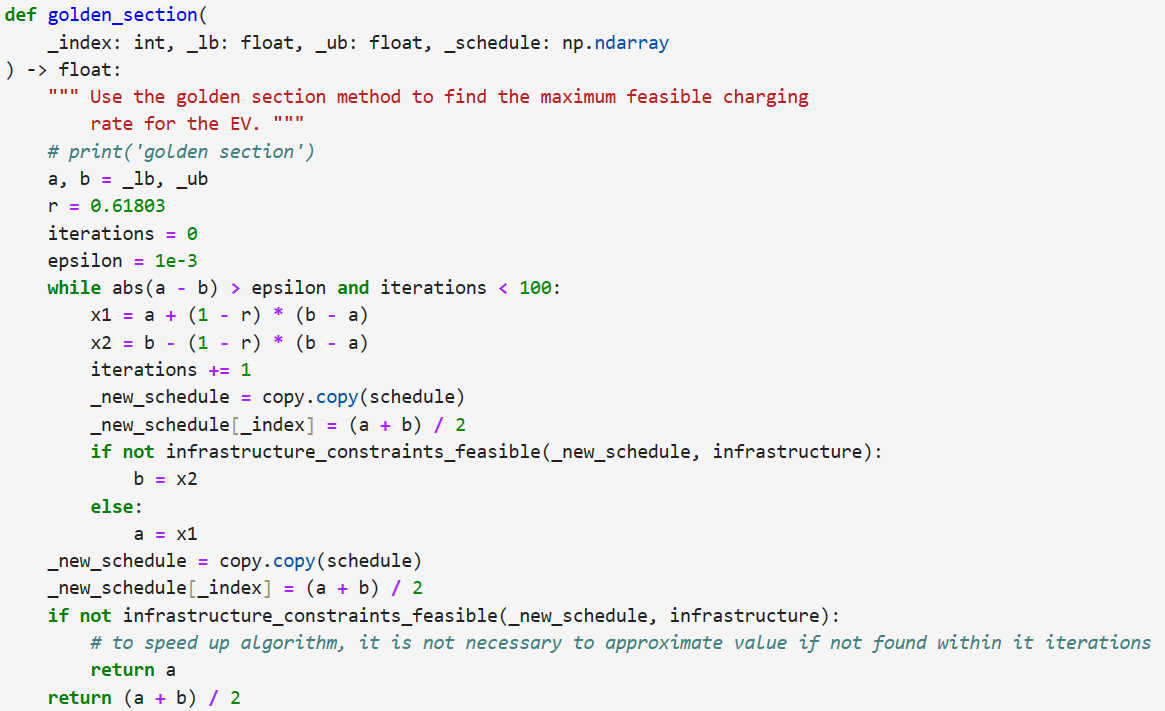
\includegraphics[width=0.8\textwidth]{images/golden_section_code.png}
    \centering
    \caption[Kód optimalizačnej metódy zlatého rezu]{Kód optimalizačnej metódy zlatého rezu.}
    \label{acndata:obr}
    \end{figure}



% should i use listing of code or just a picture of code? find out

% \begin{



